\documentclass[journal]{IEEEtran}

\usepackage{cite}
\usepackage{amsmath,amssymb,amsfonts}
\usepackage{algorithmic}

\usepackage{graphicx}
\graphicspath{{../../Dissertacao/figuras/}}

\usepackage{textcomp}
\usepackage{xcolor}
\usepackage{booktabs}                        % AAB inserido
\usepackage[utf8]{inputenc}                  % AAB inserido
\usepackage{rotating}                        % AAB inserido

\usepackage{bm,bbm}
\usepackage[binary-units]{siunitx}

\usepackage[caption=false,font=footnotesize]{subfig}
\DeclareMathOperator{\traco}{tr}



\begin{document}
\title{Fusion of Evidences in Intensities Channels for Edge Detection in PolSAR Images}
\author{Anderson A.\ de Borba, Maurício Marengoni, and Alejandro C.\ Frery,~\IEEEmembership{Senior Member,~IEEE}%
\thanks{A.\ A.\ de Borba is with the Dept.\ Engenharia Elétrica e Computação, Universidade Presbiteriana Mackenzie (UPM), and with IBMEC-SP, São Paulo, Brazil. anderson.borba@ibmec.edu.br}
\thanks{M.\ Marengoni is with the Dept.\ Engenharia Elétrica e Computação,
UPM, São Paulo, Brazil. mauricio.marengoni@mackenzie.br}
\thanks{A.\ C.\ Frery is with the Laboratório de Computação Científica e Análise Numérica (LaCCAN), Universidade Federal de Alagoas (UFAL), Maceió, Brazil. acfrery@laccan.ufal.br}}

\maketitle

\begin{abstract}
Synthetic Polarimetric Aperture Radar (PolSAR) sensors have reached an essential position in the area of remote sensing. 
The images coming from PolSAR sensors have speckle noise, making their processing and analysis challenging tasks. 
The present study discusses a detection method based on the fusion of evidence obtained in the intensity (hh), (hv), and (vv) channels of PolSAR multi-look images. 
The method consists of detecting transition points in the thinnest range of data that covers two regions using the maximum likelihood with estimates parameters from the Wishart distribution. 
The fusion methods used are the simple average, the discrete wavelet (MR-DWT), and stationary (MR-SWT) transform with multi-resolution, the principal component analysis (PCA), the ROC statistic, and a multi-resolution method based on singular values (MR-SVD). 
The results indicate an assessment of the influence of each intensity channel in the fusion of evidence with possible paths for future research.
\end{abstract}

\begin{IEEEkeywords}
PolSAR, edge detection, maximum likelihood estimation, fusion methods. 
\end{IEEEkeywords}

\section{Introduction}\label{sec_01}
\IEEEPARstart{P}{olarimetric} synthetic aperture radar (PolSAR) has achieved an essential position as a remote sensing technology. 
The data such sensors provide require specifically tailored signal processing techniques.
Among such techniques, edge detection is one of the most important operations for extracting information.
Edges are at a higher level of abstraction than mere data and, as such, provide relevant insights about the scene.

Among the available edge detection techniques for SAR and PolSAR images, it is worth mentioning:
\begin{itemize}
\item techniques based on denoising~\cite{sjx, lzly, wxbzw, law, cgaf};   
\item Markov random fields~\cite{bf};	
\item the deep learning approach~\cite{bac, ztmxzxf} applied to segmentation and classification; and,
\item statistical techniques~\cite{gmbf, fbgm, nhfc} applied in edge detection in PolSAR / SAR imagery.
\end{itemize}

This article follows the statistical modeling approach using the techniques described in~\cite{gmbf, fbgm, nhfc} to find edge evidences, followed by fusion processes~\cite{mit, bmf_2019}. 
Our approach does not attempt to reduce the speckle, but to extract information from its statistical properties.

Instead of handling fully polarimetric data, we treat each intensity channel separately, obtain evidence of edges, and then produce a single estimator of the edge position.
With this, we quantify the contribution each channel provides to the solution of the problem.

We adopted the Gambini Algorithm~\cite{gmbf_sc}, which consists in casting rays and then finding the evidence of an edge in the ray by maximizing a value function.
The value function we use is the likelihood of two samples: one inside the edge, another outside the edge.
Without loss of generality, we assume the complex scaled Wishart distribution for the fully polarimetric observations~\cite{ade}, from which Gamma laws stem for each intensity channel.
The value function depends on the estimates that index such Gamma laws.
We estimate them by maximum likelihood with the BFGS optimization method implemented in the \texttt{maxLik} package~\cite{ht}.

The value function is the total likelihood.
It is non-differentiable at most points in the domain. 
It is known that classical methods have difficulties in finding the maximum of a non-differentiable functions. 
We used the Generalized Simulated Annealing (GenSA)~\cite{xgsh} method to solve this problem. 

We discuss two fusion methods: 
MR-DWT~\cite{n_r}, and 
MR-SVD~\cite{naidu}. 
It aims to show the feasibility of a procedure for edge detection in PolSAR images. 
The objective is to understand and quantify the importance of the information provided by each channel to improve the edge detection process.

The article is structured as follows.
Section~\ref{sec_02} describes statistical modeling.
Section~\ref{sec_03} describes edge detection for PolSAR data.
Section~\ref{sec_04} describes the approach to edge evidence fusing.
Section~\ref{sec_05} presents numerical results.
Finally, Section~\ref{sec_06} concludes the work with observations, future directions of research, and the feasibility of detecting edges in each channel of PolSAR images.

\section{Statistical modeling for PolSAR data}\label{sec_02}

Multi-looked fully polarimetric data follow the Wishart distribution with PDF defined by:
\begin{equation}
    f_{\mathbf{Z}}(\mathbf{Z};\mathbf{\Sigma},L)=\frac{L^{mL}|\mathbf{Z}|^{L-m}}{|\mathbf{\Sigma}|^{L}\Gamma_m(L)} \exp(-L\traco(\mathbf{\Sigma}^{-1}\mathbf{Z})),
    \label{eq:DistWishart}
\end{equation} 
where, $\traco(\cdot)$ is the trace operator of a matrix, $\Gamma_m(L)$ is the multivariate Gamma function defined by $
	\Gamma_m(L)=\pi^{\frac{1}{2}m(m-1)} \prod_{i=0}^{m-1}\Gamma(L-i)$,
and $\Gamma(\cdot)$ is the Gamma function.
We used three $m=3$ channels in this study. 
This situation is denoted by $\mathbf{Z}\sim W(\mathbf{\Sigma}, L)$, which satisfies $E[\mathbf{Z}]=\mathbf{\Sigma}$. 
This assumption usually holds on targets where the speckle is fully developed but, since we will estimate $L$ on each sample (instead of considering the same number of looks for the whole image), we will in part take into account departures from such hypothesis.

Fully polarimetric data may be modeled by~\eqref{eq:DistWishart}.
Since we are interested in describing the information conveyed by parts of such matrix, we rely on the results presented in~\cite{lee,hsbmp}.
In particular, we assume that the distribution of each intensity channel is a 
Gamma law with probability density function
\begin{equation}
f_Z(z;\mu,L)=\frac{L^{L}z^{L-1}}{\mu^{L}\Gamma(L)} \exp\big\{-Lz/\mu\big\},\quad z>0,
\label{func_dens_uni_gamma}
\end{equation}
where $L>0$ (rather than $L\geq1$ to allow for flexibility), and
$\mu>0$ is the mean.

Given the sample $\bm z = (z_1,\dots,z_n)$,
the reduced log-likelihood of this model is
\begin{equation}
\ell(\bm z; L,\mu) = 
n \big[L\ln (L / \mu) - \ln \Gamma(L)\big]
+L \sum_{k=1}^{n}\ln z_k -\frac{L}{\mu}\sum_{k=1}^{n} z_k.
\label{eq:LogLikelihoodGamma}
\end{equation}

We obtain $(\widehat L, \widehat \mu)$, the maximum likelihood estimator (MLE) of $(L, \mu)$ based on $\bm z$, by maximizing~\eqref{eq:LogLikelihoodGamma} with the BFGS method implemented in the \texttt{maxLik} package~\cite{ht}.
We prefer optimization to solving $\nabla\ell=\bm 0$ for improved numerical stability.

\section{Edge Detection on a Single Data Strip}\label{sec_03}

We approach edge detection with the Gambini Algorithm~\cite{gmbf, fbgm, nhfc}.
%%% ACF
%This technique is convenient for our subsequent fusion step, since it provides estimates of the edge location over the same ray.
It consists of the following steps:
\begin{enumerate}
	\item Identify the centroid of a region of interest (ROI) in an automatic, semi-automatic or manual manner;
	\item cast rays from the centroid to the outside of the area;
	\item collect data on a strip, ideally of the size of a pixel, around the rays using the  Bresenham's midpoint line algorithm;
	\item compute the value function on every point of the ray;
	\item use the GenSA method~\cite{xgsh}, to find points of maxima in the functions of interest;
	\item fuse the evidence of detected edges in the (hh), (hv) and (vv) channels.
\end{enumerate}

The value function is the reduced log-likelihood of the inner and external samples of the strip denoted, respectively, as $\bm z_\text{I}$ and $\bm z_\text{E}$.
Each strip $z = (z_1,z_2,\dots,z_n)$ is, thus, partitioned in two disjoint samples at position $j$:
$$
z = (\underbrace{z_1,z_2,\dots,z_j}_{\bm z_\text{I}}, 
\underbrace{z_{j+1}, z_{j+2},\dots,z_n}_{\bm z_\text{E}}).
$$
We assume two (possibly) different models for each partition:
$\bm Z_\text{I} \sim \Gamma(\mu_\text{I},L_\text{I})$, and 
$\bm Z_\text{E} \sim \Gamma(\mu_\text{E},L_\text{E})$.
We then estimate $(\mu_\text{I},L_\text{I})$ and $(\mu_\text{E},L_\text{E})$ with $\bm z_\text{I}$ and $\bm z_\text{E}$, respectively, by maximizing~\eqref{eq:LogLikelihoodGamma}, and obtain $(\widehat{\mu}_\text{I}, \widehat{L}_\text{I})$ and $(\widehat{\mu}_\text{E}, \widehat{L}_\text{E})$.

The total log-likelihood at point $j$ is, then,
\begin{equation}\label{eq:TotalLogLikelihood}
\begin{split}
\ell(j&;\bm z_\text{I},\bm z_\text{E}) = \\
\ell(j&;\widehat{\mu}_I, \widehat{L}_I,\widehat{\mu}_E, \widehat{L}_E)=\\
&j \big[\widehat{L}_\text{I}\ln (\widehat{L}_\text{I} / \widehat{\mu}_\text{I}) - \ln \Gamma(\widehat{L}_\text{I})\big]
+\widehat{L}_\text{I} \sum_{k=1}^{j}\ln z_k -\frac{\widehat{L}_\text{I}}{\widehat{\mu}_\text{I}}\sum_{k=1}^{j} z_k +\\
&(n-j) \big[\widehat{L}_\text{E}\ln (\widehat{L}_\text{E} / \widehat{\mu}_\text{E}) - \ln \Gamma(\widehat{L}_\text{E})\big]
+\widehat{L}_\text{E} \sum_{k=j+1}^{n}\ln z_k -\\ &\frac{\widehat{L}_\text{E}}{\widehat{\mu}_\text{E}}\sum_{k=j+1}^{n} z_k.
\end{split}
\end{equation}
We then apply GenSA to find  
$$
\widehat{\jmath}= \arg\max\limits_{j\in [\min_s,N-\min_s]}\ell(j;\widehat{\mu}_I, \widehat{L}_I,\widehat{\mu}_E, \widehat{L}_E),
$$ 
where $\min_s$ is a minimum sample size that we set to $14$.

In this way, we obtain one estimates for the edge for each intensity channel.
Notice that this approach can be extended and/or modified to cope with any kind of data.

We will see ways of fusing these evidences in the next section.

\section{Fusion of Evidences}\label{sec_04}

Denote in the following $\widehat{\bm\jmath}_c$ the binary image with same support as the input data $c$, where $1$ denotes an estimate of edge and $0$ otherwise.
We have $n_c$ of these image to fuse, and the result of the fusion will be denoted $\text{I}_F$.

We compare the results of six fusion techniques, namely:
simple average, 
multi-resolution discrete wavelet transform (MR-DWT),
principal components analysis (PCA), 
ROC statistics,
multi-resolution stationary wavelet transform (MR-SWT), and
multi-resolution singular value decomposition (MR-SVD).

%The estimated evidence image and the fusion image are defined to perform the fusion techniques. The first can be defined as $\widehat\jmath_c(x,y)$, where $x$ and $y$, indicate the range of pixels in an image equal in size to the data image chosen for analysis. The image is binary, where the value one is put on the pixel estimated as edge evidence by the MLE method, and zero on the other pixels, for each channel. The second called $\text{I}_F(x,y)$ is the result of the fusion method. 

%Refs.~\cite{bmf_2019,n_r,mit,gs,fawcett} provide details about the three first.
%We describe the two latter below.

\subsection{Simple average}
The simple average fusion method proposes the arithmetic mean of the edge evidence in each of the $n_c$ channels:
$\text{I}_F(x,y)=(n_c)^{-1}\sum_{c=1}^{n_c} \widehat{\bm\jmath}_c(x,y)$.
%where $\widehat\jmath_c$ denotes the estimate obtained in channel $c$.

\subsection{Multi-Resolution Discrete Wavelet -- MR-DWT} 
This section is based on~\cite{n_r}.
%We apply DWT filters separately in the vertical and horizontal directions of each image $\bm{\widehat\jmath}_c$, then down-sampled by a factor of two. 
%In this way, each image is filtered by the low pass filter $\text{L}$ in the vertical direction and the high pass filter $\text{H}$ in the horizontal direction, then down-sampled to create the matrices coefficients  $\bm{\widehat\jmath}_{c\text{L}}$ and $\bm{\widehat\jmath}_{c\text{H}}$.
We apply DWT filters for each the binary image $\bm{\widehat\jmath}_c$, the images are filtered by low pass filter $\text{L}$ in the vertical direction and high pass filter $\text{H}$ in the horizontal direction, then down-sampled to create the coefficient matrices $\bm{\widehat\jmath}_{c\text{L}}$ and $\bm{\widehat\jmath}_{c\text{H}}$.
These operations are repeated for the coefficient matrices, leading to $\bm{\widehat\jmath}_{c\text{LL}}$, $\bm{\widehat\jmath}_{c\text{LH}}$, $\bm{\widehat\jmath}_{c\text{HL}}$, and $\bm{\widehat\jmath}_{c\text{HH}}$, and so on achieving successive resolution levels.

%%% ACF Detalhar as operações usando a notação acima: a média é pixel-a-pixel? quais bandas são promediadas?
%%% AAB A média é pixel a pixel. Todas as bandas são usadas na média. Vou tentar deixar claro no texto. Creio que respondi no item 2 abaixo.
%%% AAB Eu entendo que investigar outros tipo de ponderação (suprimir canais, por exemplo) pode ser realizado. Ainda não consegui fazer esses testes.
%%% AAB O nivel de resolução que uso é 1, esse é outro ponto de investigação, seria interessante aumentar esse nível e ver o que acontece na fusão. Tb não consegui realizar esses teste. Inseri no item 1) abaixo a info sobre o nível de resolução.
The DWT fusion method has the following steps:
\begin{enumerate}
\item Calculate the DWT decomposition by getting $\bm{\widehat\jmath}_{c\text{LL}}$, $\bm{\widehat\jmath}_{c\text{LH}}$, $\bm{\widehat\jmath}_{c\text{HL}}$, and $\bm{\widehat\jmath}_{c\text{HH}}$, for each channel. In this work is used one resolution level;
\item in the decomposition $\bm{\widehat\jmath}_{c\text{HH}}$, the arithmetic mean of all channels are computed, pixel by pixel, and in the decomposition $\bm{\widehat\jmath}_{c\text{LL}}$, $\bm{\widehat\jmath}_{c\text{LH}}$, $\bm{\widehat\jmath}_{c\text{HL}}$, the maximum is found among all channel, pixel by pixel, finding a new operators $\bm{\bar\jmath}_{c\text{LL}}$, $\bm{\bar\jmath}_{c\text{LH}}$, $\bm{\bar\jmath}_{c\text{HL}}$, and $\bm{\bar\jmath}_{c\text{HH}}$;
\item used these operators, the image with the fusion of edge evidence $\text{I}_F(x, y)$ is computed performing the inverse DWT transformation.
\end{enumerate}

\subsection{Principal component analysis -- PCA}

This section is based on~\cite{n_r,mit}.
The method is comprised of the following steps:
\begin{enumerate}
\item organize the data in such a way that $\bm{\widehat\jmath}_c$ is a column vector, forming a Y matrix of dimension $\ell\times nc$, where $\ell=m\cdot n$, the lines times the columns of $\bm{\widehat\jmath}_c$;
\item calculate the average of the elements of these columns, generating a vector dimension of $1\times nc$;
\item subtract the average of each column from the Y matrix, resulting a matrix of the same dimension X; 
\item find C, the covariance matrix of X, with dimensions $nc\times nc$;
\item compute the eigenvalues $\Lambda$ and eigenvectors V of C, and sort the eigenvalues and eigenvectors in descending order. %The matrices generated by the eigenvalues, on the principal diagonal, and the eigenvectors placed in columns;
\item compute the components $\text{P}_c=\frac{\text{V}_c}{\sum_{c=1}^{nc} \text{V}_c}$. %with $i=1,\dots,nc$;
\item fuse $\text{I}_F(x,y)=\sum_{c=1}^{nc}\text{P}_c\bm{\widehat\jmath}_c(x,y)$, recalling that $\sum_{c=1}^{nc}\text{P}_c=1$.
\end{enumerate}

\subsection{ROC statistics}

The ROC method was proposed and described on~\cite{gs,fawcett}:
\begin{enumerate}
%\item the evidence of edges in each channels $\bm{\widehat\jmath}_c$, with $c=1,\dots,nc$ in a binary way;
\item define a V edge frequency matrix. The V matrix is generated by adding the evidence of $\bm{\widehat\jmath}_c$ matrices;
\item use thresholds ranging from $t=1,\dots,nc$ generating $\text{M}_t$ matrices;
\item compare each $\text{M}_t$ fixed with all $\bm{\widehat\jmath}_c$, find the confusion matrix to generate the ROC curve. The point of the ROC curve closest (in the sense of the Euclidean distance) to the diagnostic line will have its threshold considered optimal;
\item the $\text{M}_t$ matrix which corresponds to the threshold closest to the diagnostic line is the result of the fusion.
\end{enumerate}

\subsection{Multi-Resolution Stationary Wavelet Transform -- MR-SWT}  
This section is based on~\cite{n_r, jjly}. The difference between MR-DWT and MR-SWT method is in the replacement of the filters used in the DWT by the filters used in the SWT.

\subsection{Multi-Resolution Singular Value Decomposition -- MR-SVD}

MR-SVD Fusion~\cite{naidu} works similar to the MR-DWT method. The difference consists in changing the DWT filters by the SVD filters. The MR-SVD fusion method can be summarized as follows:
\begin{enumerate}
%\item Organize the binary image $\bm{\widehat\jmath}_c$ in matrices $\text{X}_\ell$ with dimension $4\times\frac{\text{M}}{2}\frac{\text{N}}{2}$ according to~\cite{naidu}, where M is the number of rows and N is the number of columns in $\bm{\widehat\jmath}_c$, and $\ell$ is the level resolution to set. In this work is used one resolution level;
\item Organize the binary image $\bm{\widehat\jmath}_c$ in matrices into non-overlapping $2\times 2$ blocks and arrange each block into a $4\times 1$ vector by stacking columns to form the data matrix $\text{X}_\ell$, where M is the number of rows and N is the number of columns in $\bm{\widehat\jmath}_c$, and $\ell$ is the level resolution to set. In this work is used one resolution level;
\item find the SVD decomposition to matrix $\text{T}=\text{X}_\ell \text{X}_\ell^\text{T}=\text{U}_\ell \text{S}^2 \text{U}_\ell^T$, where $s(1)\geq s(2) \geq s(3) \geq s(4)$ compose the singular value matrix S, and U is an real or complex unitary matrix;
\item put $\widehat{\text{X}}_\ell=\text{U}_\ell^T\text{X}_\ell$ and transform the lines on this matrix in new matrices with dimensions $\frac{\text{M}}{2}\times\frac{\text{N}}{2}$, named respectively $\{\Phi_\ell, \Psi_\ell^\text{V}, \Psi_\ell^\text{H}, \Psi_\ell^\text{D}\}$. In the next level decomposition, the $\text{X}_\ell$ is replaced by $\Phi_\ell$ until the level L is reached. The MR-SVD method is represented as:
\begin{equation}\label{msvd_iter}
\widehat{\text{X}}\leftarrow \left\{\Phi_L,\{\Psi_\ell^\text{V},\Psi_\ell^\text{H},\Psi_\ell^\text{D} \}_{\ell=1}^L,\{\text{U}_\ell\}_{\ell=1}^L \right\}
\end{equation}
\item once the SVD is applied to level $\ell$ the fusion process is executed as follow: In the operators $\Psi_\ell^\text{V}$, $\Psi_\ell^\text{H}$ and $\Psi_\ell^\text{D}$, the maximum is found among all channel, pixel by pixel, resulting in new operators $\bar{\Psi}_\ell^\text{V}$, $\bar{\Psi}_\ell^\text{H}$ and $\bar{\Psi}_\ell^\text{D}$. The operators $\Phi_L$, and $\text{U}_\ell$ are averaged over all the channels, pixel by pixel;
\item the image with the fusion of edge evidence $\text{I}_F(x,y)$ is performed with the SVD transformation for each level $\ell$. 
\end{enumerate}
\section{Numerical results}\label{sec_05}

\subsection{Real PolSAR image}
The PolSAR image of the Flevoland region in the Netherlands is used for the numerical tests. 
Fig.~(\ref{flevoland_radial_4look}) shows the ROI, with the radial lines for edge detection. The Flevoland image has dimension ($750\times 1024$) pixels.

\begin{figure}[hbt]
\centering
	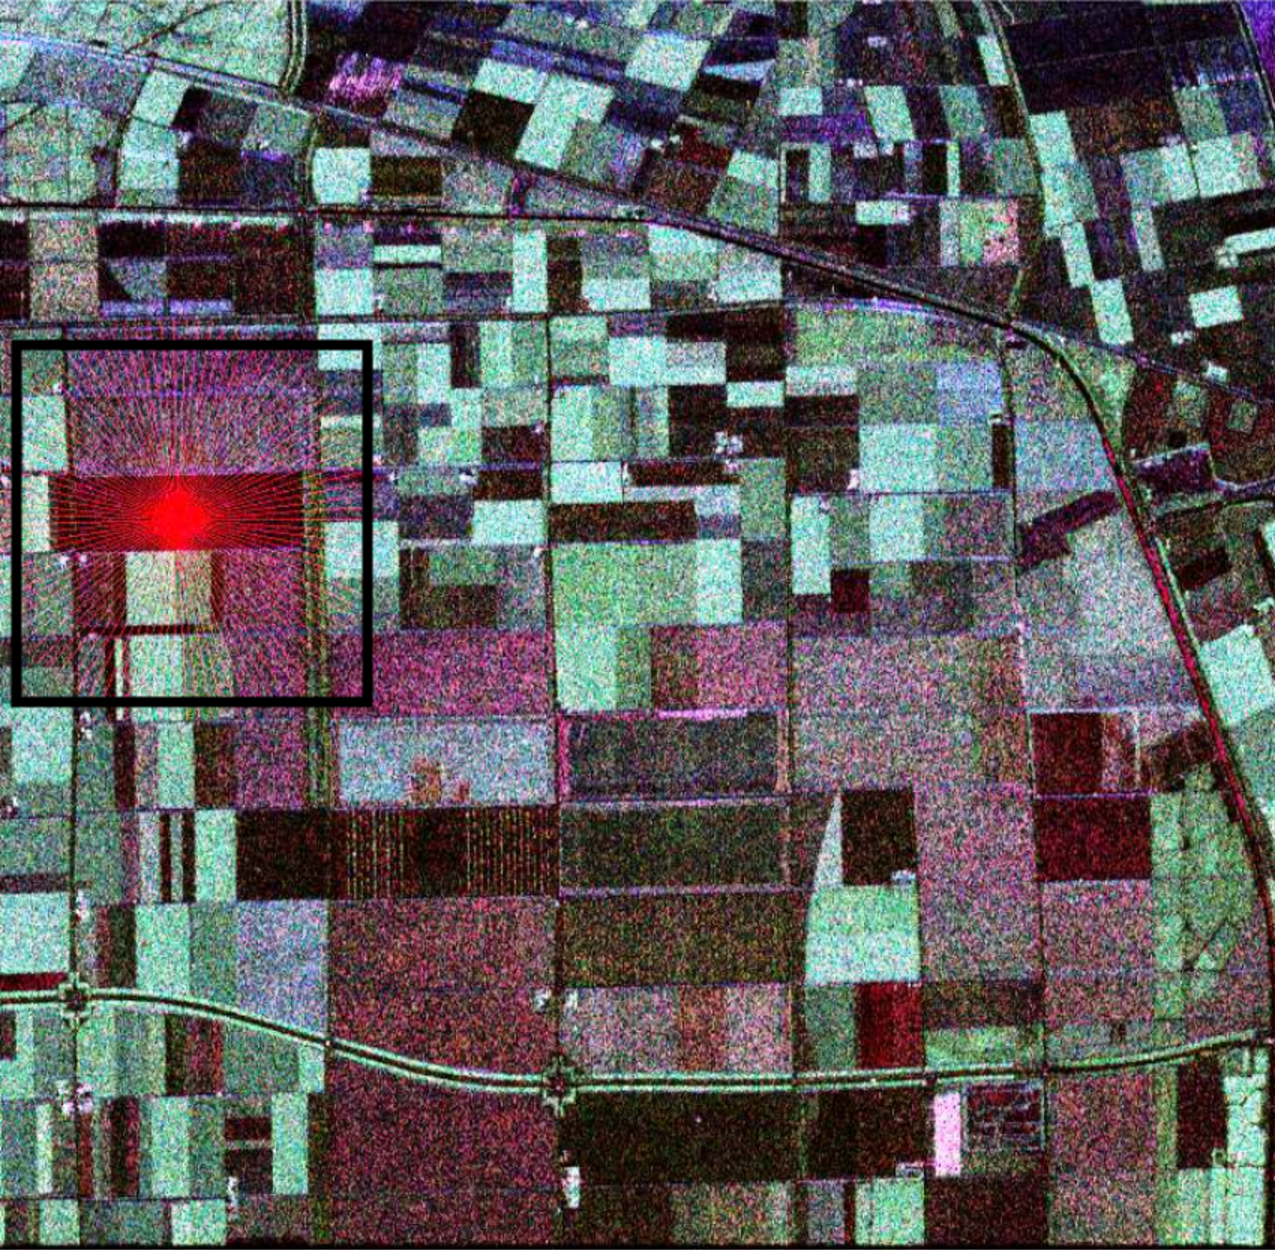
\includegraphics[width=\linewidth]{flevoland_radial_4_look_black}
	\caption{ROI in the image of Flevoland.}
\label{flevoland_radial_4look}
\end{figure}

The estimates from equation~\eqref{eq:LogLikelihoodGamma} is used in equation~\eqref{eq:TotalLogLikelihood} generating an oscillation at the end of each radial line, depending on the radial considered. In order to get around this problem, in this PolSAR image, 14 pixels on each side of radial lines were not considered. The number of pixel were determined empirically.

Figs.~\ref{evidencias_hh_hv_vv}\subref{evidencias_hh_hv_vv:a}, \subref{evidencias_hh_hv_vv:b} and~\subref{evidencias_hh_hv_vv:c} show, respectively, the edge evidence in the $\text{hh}$, $\text{hv}$ and $\text{vv}$ channels. For each of these images, the MLE is executed.

It is worth noting that GenSA has accurately identified the maximum value of function $\ell(j)$, even in the presence of multiple local maxima. Another important observation concerns the performance of the proposed method in the $\text{hv}$ channel. The method presents a few outliers points, and, good accuracy in the detection edges evidence. The method presents the best performance when compared to channels $\text{hh}$ and $\text{vv}$. 
   \begin{figure*}[hbt]
	\centering
     \subfloat[Evidences in channel $\text{hh}$ \label{evidencias_hh_hv_vv:a}]{%
       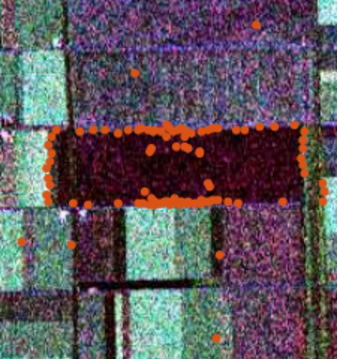
\includegraphics[width=0.32\linewidth]{flevoland_hh_evid_param_L_mu_14_pixel_crop}
     }
     \subfloat[Evidences in channel $\text{hv}$ \label{evidencias_hh_hv_vv:b}]{%
       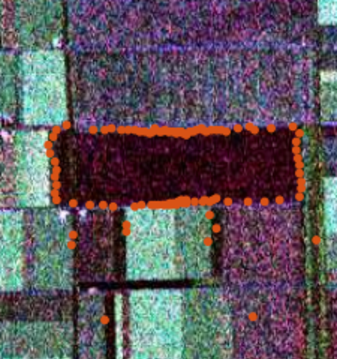
\includegraphics[width=0.32\linewidth]{flevoland_hv_evid_param_L_mu_14_pixel_crop}
     }
     \subfloat[Evidences in channel $\text{vv}$ \label{evidencias_hh_hv_vv:c}]{%
       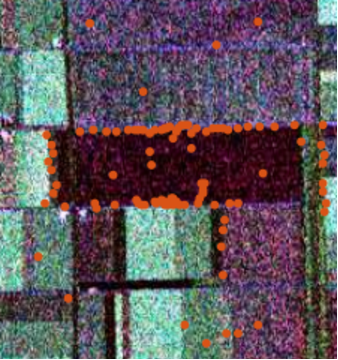
\includegraphics[width=0.32\linewidth]{flevoland_vv_evid_param_L_mu_14_pixel_crop}
     }
     \caption{Edges evidences 14 pixel range}
     \label{evidencias_hh_hv_vv} 
   \end{figure*}

Figs.~\ref{fusion_met}\subref{fusion_met:a},~\subref{fusion_met:b},~\subref{fusion_met:c},~\subref{fusion_met:d},~\subref{fusion_met:e}, and~\subref{fusion_met:f} show the results of fusing these evidences. 

The simple average and PCA methods have similar performances to indicate pixels as edges. The time to perform the methods is shown in the table~(\ref{metrica_de_tempo}). Thus, one can see that the time for the PCA method is 2.19 times longer than the simple average.  

The MR-SVD method shows excellent performance to indicate pixels of edges; the number of pixels outliers is much smaller than the other methods. The significant disadvantage of the MSVD method is the runtime. Table~(\ref{metrica_de_tempo}) shows that it has the highest time.

The ROC Fusion shown edge pixels with good accuracy and a small number of outliers, but it doesn't show pixels that are edges. One way to get around this problem would be to increase the number of channels considered using other PDF.

The post-processing is an option to be used in all the fusion methods. An idea can be found in Ref.~\cite{fbgm}. 

\begin{figure*}[hbt]
	\centering
     \subfloat[Average fusion\label{fusion_met:a}]{%
       %\includegraphics[width=0.2\textwidth]{example-image-a}
       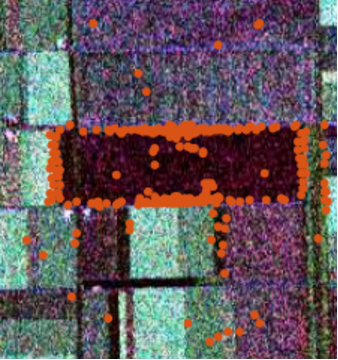
\includegraphics[width=0.32\linewidth]{flevoland_fus_media_param_L_mu_14_pixel_crop}
     }
     \subfloat[DWT fusion\label{fusion_met:b}]{%
       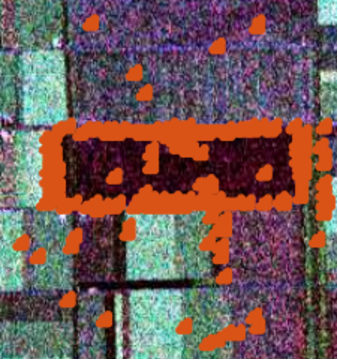
\includegraphics[width=0.32\linewidth]{flevoland_fus_dwt_param_L_mu_14_pixel_crop}
     }
     \subfloat[PCA fusion \label{fusion_met:c}]{%
       %\includegraphics[width=0.2\textwidth]{example-image-a}
       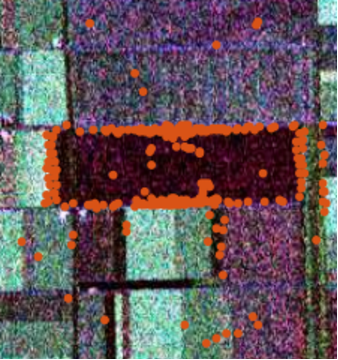
\includegraphics[width=0.32\linewidth]{flevoland_fus_pca_param_L_mu_14_pixel_crop}       
     }\\
     \subfloat[ROC fusion\label{fusion_met:d}]{%
       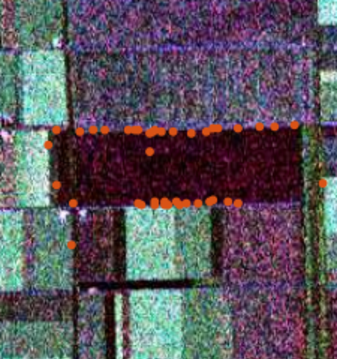
\includegraphics[width=0.32\linewidth]{flevoland_fus_roc_param_L_mu_14_pixel_crop}
     }
     \subfloat[SWT fusion\label{fusion_met:e}]{%
       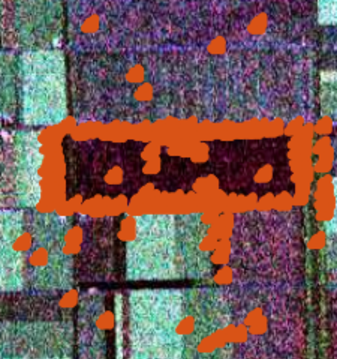
\includegraphics[width=0.32\linewidth]{flevoland_fus_swt_param_L_mu_14_pixel_crop}
     }
     \subfloat[MSVD fusion\label{fusion_met:f}]{%
       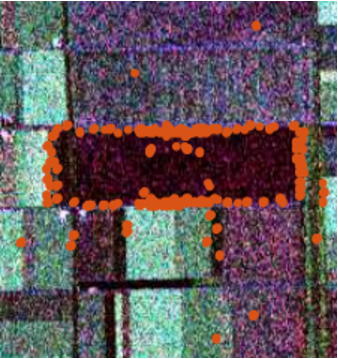
\includegraphics[width=0.32\linewidth]{flevoland_fus_svd_param_L_mu_14_pixel_crop}
     }
     \caption{Results of applying the five fusion methods}
     \label{fusion_met}
\end{figure*}

\subsection{Implementation Details}
The system presented here was executed on a Intel\copyright\ Core i7-9750HQ CPU \SI{2.6}{\giga\hertz} \SI{16}{\giga\byte} RAM computer.  
The method for detecting edge evidence MLE was implemented in R language; on the other hand, the fusion methods were implemented in Matlab language. 
%Table~\ref{metrica_de_tempo} shows the computational cost of each of the fusion methods.

\subsection{Processing times} 

This section presents a table of the processing time to fusion's methods. The measurement of time was performed only for the fusion method, disregarding the time for the method that finds the evidence of edges, because it is the same for all fusion methods. The measurement was performed by running the fusion method 20 times and performing the average of these times. The result is shown in the first row of the table (\ref{metrica_de_tempo}), the second row of the table  (\ref{metrica_de_tempo}) was constructed by choosing the shortest time of the methods as the reference time (TR) that shows how longer the others methods are.
\begin{table}[hbt]
	\centering
	\tiny
	\caption{System performance.}\label{metrica_de_tempo}
\begin{tabular}{@{}lllllll@{}} \toprule
	Method       & Average    &   PCA      &  ROC      & DWT       &  SWT        &  MSVD \\ \midrule
	Time (s)      & 0.00858185 & 0.01880955 &0.39989020 &0.07938820 &  0.18071635 & 1.11195710  \\
    Ref. time     & TR & 2.19TR &46.59TR & 9.25TR   & 21.05TR & 129.57TR  \\ \bottomrule
\end{tabular}
\end{table}
\section{Conclusion}\label{sec_06}

Initially, evidence of edges was found using the maximum likelihood method and BFGS to estimate the $L$ and $\mu$ parameters. Later this parameter was used in the maximum likelihood method; at this point, the GenSA method for estimation of edge evidence were applied. In the article, three intensity channels are used to apply the maximum likelihood methods showing excellent accuracy on the actual image of a Flevoland region. The maximum likelihood method in the (hv) channel has superior performance compared to (hh) and (vv) channels.

It is essential to point out that the maximum likelihood method when inserting the $L$ and $\mu$ parameters results in a non-smooth function presenting many local maxima. The difficulty of using the classical optimization methods in this kind function is known, then to get around this problem the simulated annealing method was applied because it is appropriate to optimize non-differentiate functions.

The fusion methods like simple average, MR-DWT, PCA, ROC, MR-SWT, and MR-SVD were applied to the results of the maximum likelihood methods on each channel. The purpose of applying the fusion methods was to obtain better edge detection accuracy and measure the importance of each channel in the final fusion result. On this sense are can notice that mainly the (vv) channel did not contribute to get a good accuracy of the fusion methods.

From the obtained results, the feasibility of procedure proposes for edge detection in PolSAR images is shown.

Finally, three observations are highlighted on future work; the ROC statistic can be improved by increasing the number of PDF for the intensity channels, the weight adjustment for the channels or the choice of the best channels for the fusion of edge evidence, and the use of post-processing on the images coming from the fusion.

\bibliographystyle{IEEEtran}
\bibliography{../../../Text/bibliografia}
\end{document}

